\documentclass{article}
\usepackage{amsmath}
\usepackage{amssymb}
\usepackage{graphicx}
\usepackage{hyperref}
\usepackage[version=4]{mhchem}


\begin{document}
(AMC) In the accompanying figure, segments \(A B\) and \(C D\) are parallel, the measure of angle \(D\) is twice that of angle \(B\), and the measures of segments \(A D\) and \(C D\) are \(a\) and \(b\) respectively. Then the measure of \(A B\) is equal to\\
(A) \(\frac{1}{2} a+2 b\)\\
(B) \(\frac{3}{2} b+\frac{3}{4} a\)\\
(C) \(2 a-b\)\\
(D) \(4 b-\frac{1}{2} a\)\\
(E) \(a+b\).\\
\centering
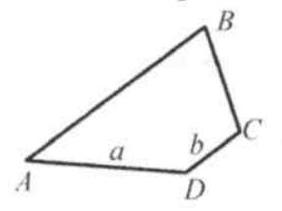
\includegraphics[width=\textwidth]{images/110(3).jpg}

Solution: (E).\\
Method 1:\\
Let the bisector of \(\angle D\) intersect \(A B\) at \(E\) (see figure). Then the alternate interior angles \(A E D\) and \(E D C\) as well as \(\angle A D E\) are equal to angle \(B\), so \(\triangle A E D\) is isosceles with equal angles at \(P\) and \(D\). This means that \(A E=A D=a\).

Since \(E B C D\) is a parallelogram, we have \(E B=D C=b\); so \(A B\)\\
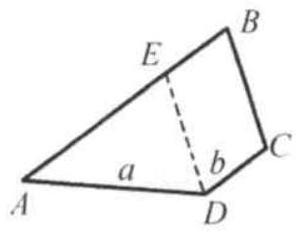
\includegraphics[width=\textwidth]{images/110(2).jpg} \(=A E+E B=a+b\).

Method 2:\\
Extend \(D C\) to \(E\) and connect \(B E\). This results in \(A B E D\) being a parallelogram, and so \(A B=D E, B E=a\), and \(\angle A D C=\) \(\angle A B E\).\\
\centering
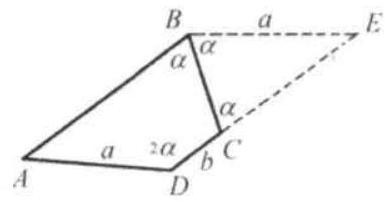
\includegraphics[width=\textwidth]{images/110(1).jpg}


Since \(\angle A B C=\alpha\), then \(\angle C B E=\alpha\). Since \(\mathrm{AB} / / \mathrm{DE}, \angle E C B=\angle E B C\). Thus, \(B E=\) \(E C=a\), and so \(A B=a+b\).

Method 3:\\
Draw \(E C / / A D\) to meet \(A B\) at \(E\). This gives us parallelogram \(A E C D\) where \(A D=E C=a\) and \(\angle A D C=\angle A E C\).\\
Since \(\angle A E C=2 \alpha=\angle E B C+\angle E C B\), so \(\angle E C B=\alpha\). Thus,\\
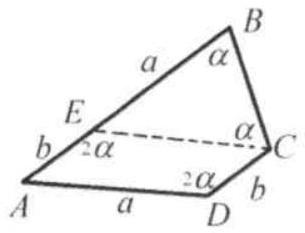
\includegraphics[width=\textwidth]{images/111.jpg} \(B E=E C=a\), and so \(A B=a+b\).


\end{document}
